\section[Руководство пользователя]{РУКОВОДСТВО ПОЛЬЗОВАТЕЛЯ}

\subsection{Просмотр каталога велосипедов}

Страница \textit{catalog.jsp} является главной страницей разрабатываемого сайта.
Таким образом для просмотра каталога доступных велосипедов необходимо перейти
по адресу \textit{localhost:8080/catalog}. При попытке попасть на сайт по адресу
\textit{bikeshop.by} пользователь будет перенаправлен на страницу каталога.

Страница каталога предоставляет пользователю краткую характеристику велосипеда.
Просмотр полной характеристики доступен для каждого велосипеда.
Вид страницы \textit{catalog.jsp} представлен на рисунке~\ref{fig:catalog_jsp}.

\begin{figure}[h]
  \centering
  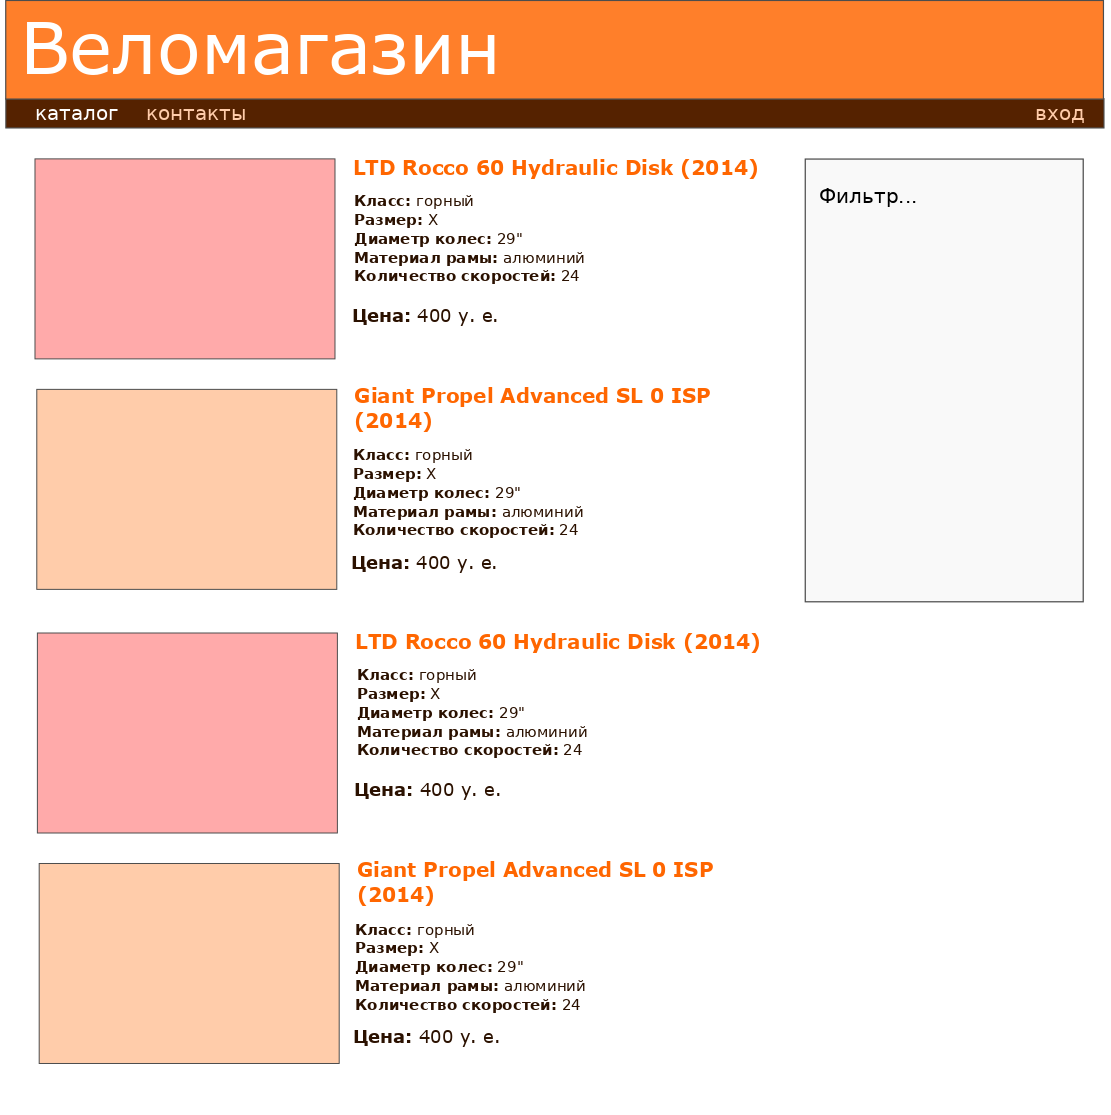
\includegraphics[width=130mm]{pic/catalog_template.png}
  \caption{Внешний вид страницы \textit{catalog.jsp}}
  \label{fig:catalog_jsp}
\end{figure}

\pagebreak

При щелчке мыши по области, содержащей краткое описание велосипеда,
будет осуществлён переход на страницу с подробным описанием выбранного товара,
изображенную на рисунке~\ref{fig:detail_jsp}.

\begin{figure}[h]
  \centering
  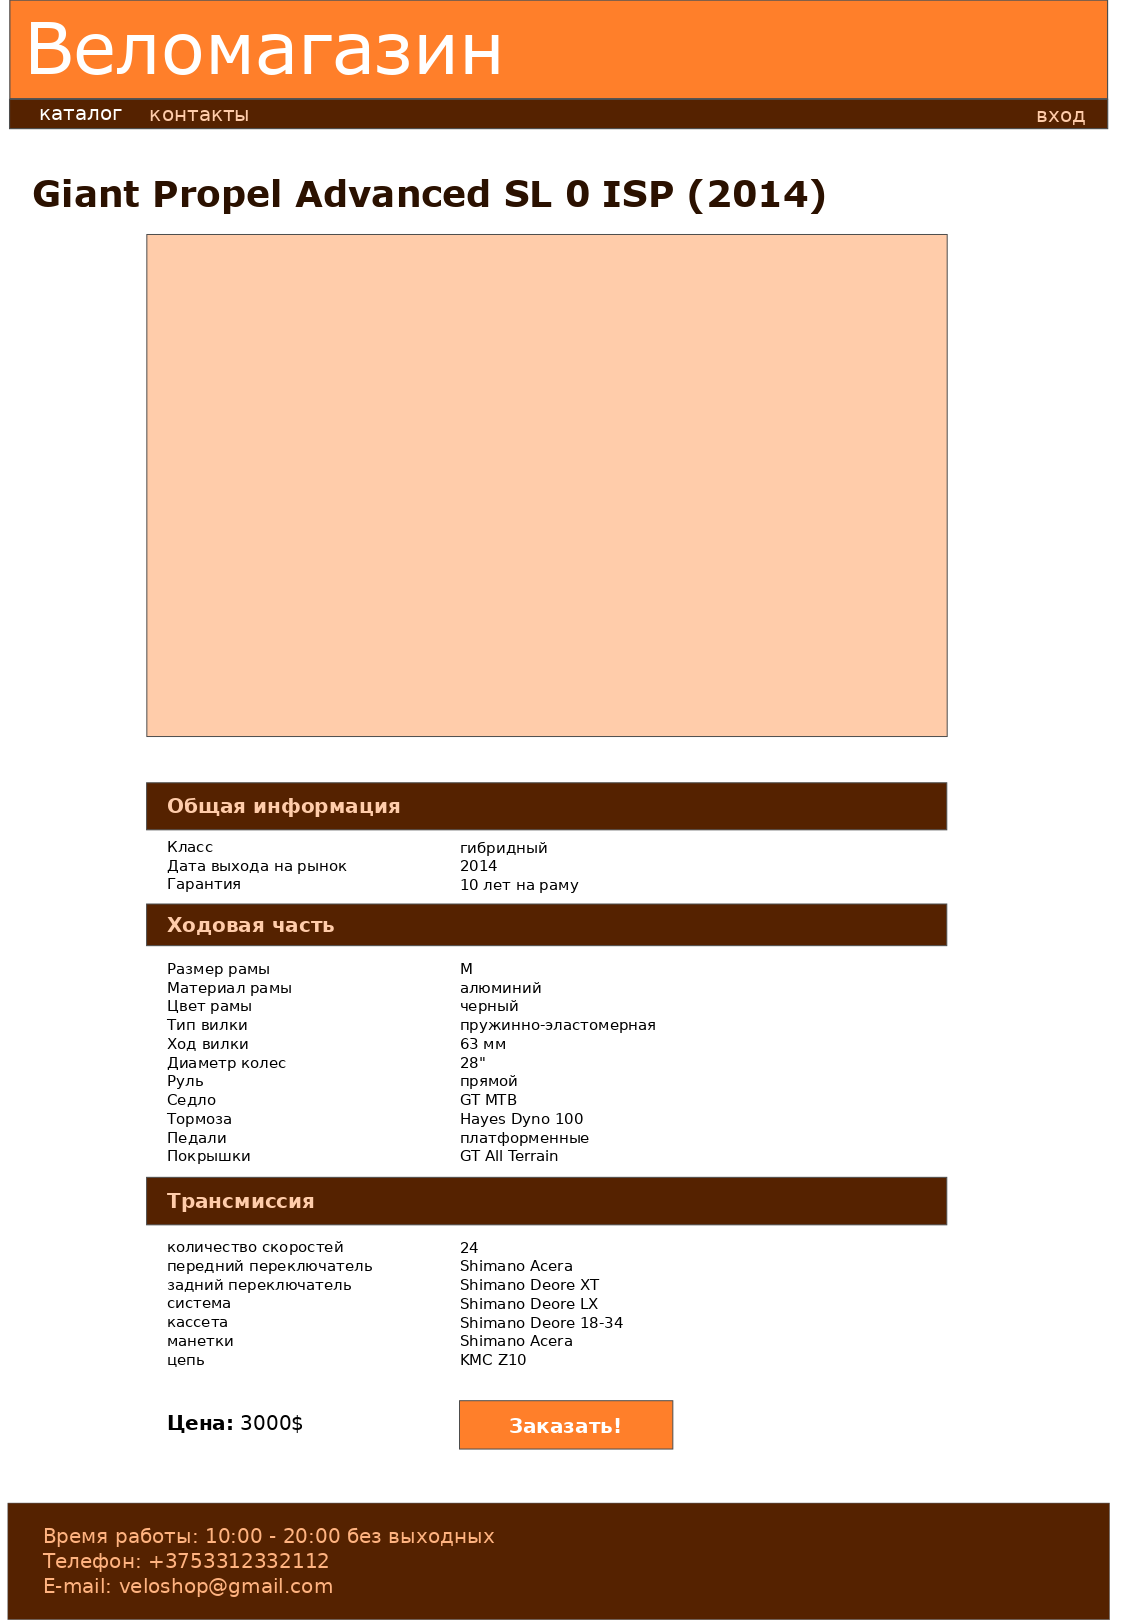
\includegraphics[width=125mm]{pic/detail_template.png}
  \caption{Внешний вид страницы \textit{detail.jsp}}
  \label{fig:detail_jsp}
\end{figure}

\pagebreak

\subsection{Покупка велосипеда}

Для покупки велосипеда необходимо перейти на страницу с подробным описанием
велосипеда и нажать кнопку <<Заказать!>>. После этого откроется форма для заполнения
контактных данных пользователя, проиллюстрированная на рисунке~\ref{fig:order_jsp}.

\begin{figure}[h]
  \centering
  
\includegraphics[width=150mm]{pic/order_template.png}
  \caption{Внешний вид страницы \textit{order.jsp}}
  \label{fig:order_jsp}
\end{figure}

В том случае, если пользователь авторизован, контактные данные покупателя
будут автоматически заполнены.

После заполнения формы контактных данных для заказа велосипеда необходимо нажать на кнопку
\textit{<<Подтвердить заказ>>}. Таким образом велосипед поступает в очередь на обработку
заказов.

\pagebreak

\subsection{Страница пользователя}

После успешной авторизации пользователя на сайте, он может посетить свою страницу.
На ней можно просмотреть весь список покупок конкретного пользователя.
Пример отображения страницы <<user.jsp>> приведен на рисунке~\ref{fig:user_jsp}.

\begin{figure}[h]
  \centering
  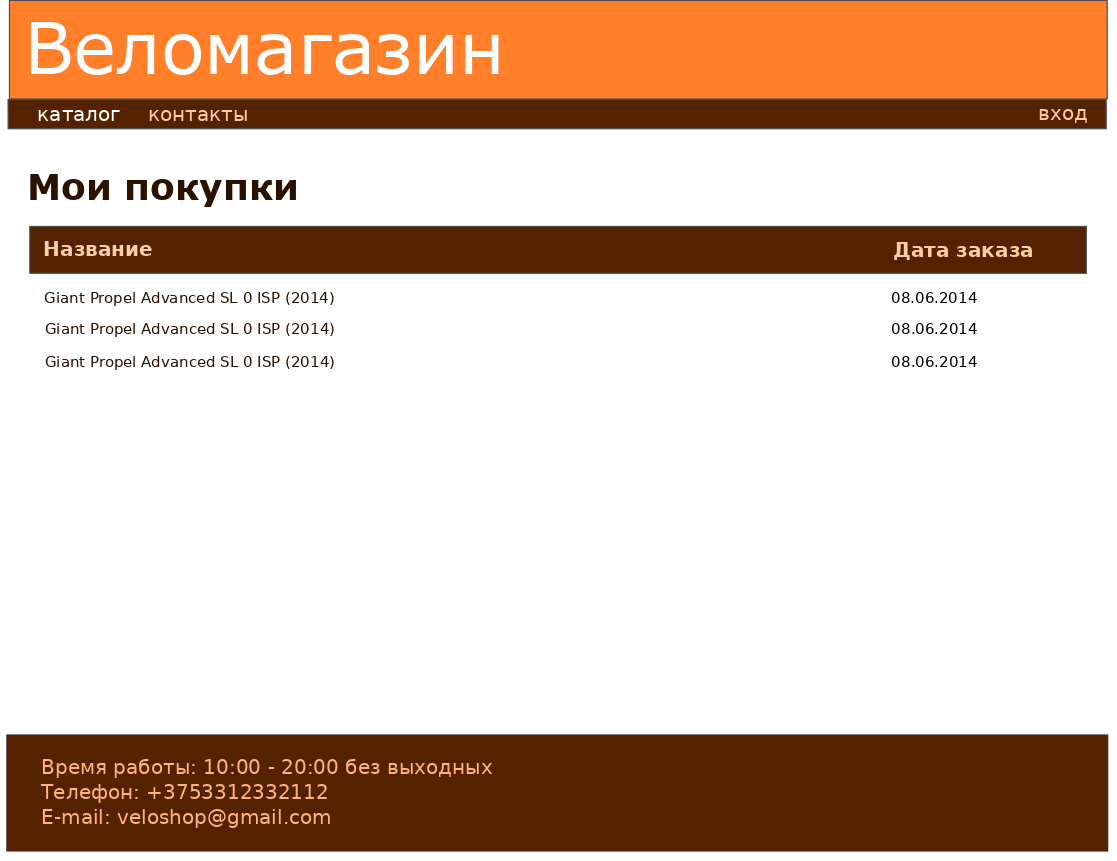
\includegraphics[width=150mm]{pic/user_template.png}
  \caption{Внешний вид страницы \textit{user.jsp}}
  \label{fig:user_jsp}
\end{figure}

\subsection{Страница администратора}

В том случае, если авторизованный по имеет привилегии администратора, сайт
изменяет свой функционал, расширяя его страницей администратора. На странице
администратора имеется возможность выполнить CRUD-операции для таблиц, а также
экспортировать и импортировать товар в формат xml.

\pagebreak

Администратор обязан управлять заказами, поэтому для него доступна страница
обработки заказов, изображенная на рисунке~\ref{fig:order-processing_jsp}.

\begin{figure}[h]
  \centering
  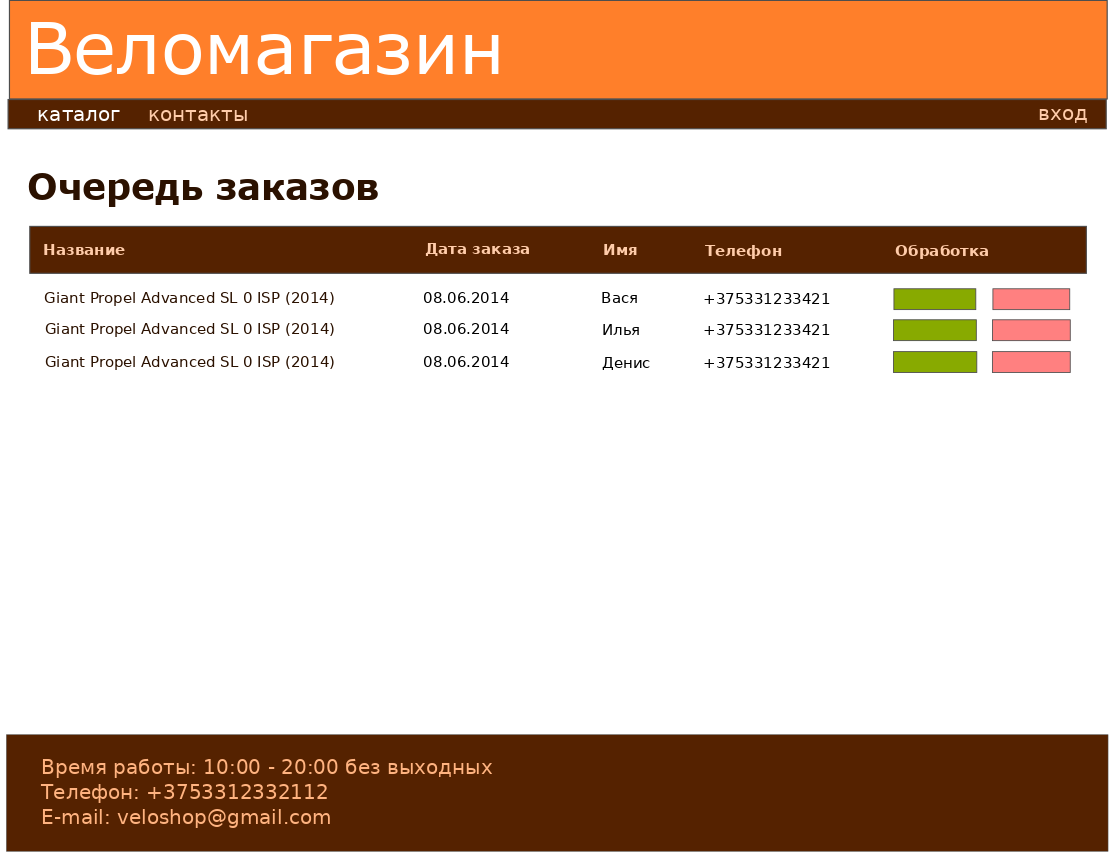
\includegraphics[width=160mm]{pic/order_processing_template.png}
  \caption{Внешний вид страницы \textit{order-processing.jsp}}
  \label{fig:order-processing_jsp}
\end{figure}

\pagebreak
